%\RequirePackage{currfile}
\documentclass[12pt]{beamer}
\usepackage[utf8]{inputenc}
\usepackage[spanish]{babel}
\usepackage{standalone}
\usepackage{color}
\usepackage{siunitx}
\usepackage{hyperref}
\usepackage[outdir=./]{epstopdf}
%\hypersetup{colorlinks,linkcolor=,urlcolor=blue}
%\hypersetup{colorlinks,urlcolor=blue}
\usepackage{xcolor,soul}
\usepackage{etoolbox}
\usepackage{amsmath}
\usepackage{amsthm}
\usepackage{mathtools}
\usepackage{tcolorbox}
\usepackage{physics}
\usepackage{multicol}
\usepackage{bookmark}
\usepackage{longtable}
\usepackage{listings}
\usepackage{cancel}
\usepackage{wrapfig}
\usepackage{empheq}
\usepackage{graphicx}
\usepackage{tikz}
\usepackage{tikz-3dplot}
\usetikzlibrary{calc, patterns, matrix, backgrounds, decorations,shapes, arrows.meta}
\usepackage[autostyle,spanish=mexican]{csquotes}
\usepackage[os=win]{menukeys}
\usepackage{pifont}
\usepackage{pbox}
\usepackage{bm}
\usepackage{caption}
\captionsetup{font=scriptsize,labelfont=scriptsize}
%\usepackage[sfdefault]{roboto}  %% Option 'sfdefault' only if the base font of the document is to be sans serif

%Sección de definición de colores
\definecolor{ao}{rgb}{0.0, 0.5, 0.0}
\definecolor{bisque}{rgb}{1.0, 0.89, 0.77}
\definecolor{amber}{rgb}{1.0, 0.75, 0.0}
\definecolor{armygreen}{rgb}{0.29, 0.33, 0.13}
\definecolor{alizarin}{rgb}{0.82, 0.1, 0.26}
\definecolor{cadetblue}{rgb}{0.37, 0.62, 0.63}
\definecolor{deepblue}{rgb}{0,0,0.5}
\definecolor{brown}{rgb}{0.59, 0.29, 0.0}
\definecolor{OliveGreen}{rgb}{0,0.25,0}
\definecolor{mycolor}{rgb}{0.122, 0.435, 0.698}

\newcommand*{\boxcolor}{orange}
\makeatletter
\newcommand{\boxedcolor}[1]{\textcolor{\boxcolor}{%
\tikz[baseline={([yshift=-1ex]current bounding box.center)}] \node [rectangle, minimum width=1ex, thick, rounded corners,draw] {\normalcolor\m@th$\displaystyle#1$};}}
 \makeatother

 \newcommand*\widefbox[1]{\fbox{\hspace{2em}#1\hspace{2em}}}

\newtcbox{\mybox}{on line,
  colframe=mycolor,colback=mycolor!10!white,
  boxrule=0.5pt,arc=4pt,boxsep=0pt,left=6pt,right=6pt,top=6pt,bottom=6pt}

\usefonttheme[onlymath]{serif}
%Sección de definición de nuevos comandos

\newcommand*{\TitleParbox}[1]{\parbox[c]{1.75cm}{\raggedright #1}}%
\newcommand{\python}{\texttt{python}}
\newcommand{\textoazul}[1]{\textcolor{blue}{#1}}
\newcommand{\azulfuerte}[1]{\textcolor{blue}{\textbf{#1}}}
\newcommand{\funcionazul}[1]{\textcolor{blue}{\textbf{\texttt{#1}}}}
\newcommand{\ptilde}[1]{\ensuremath{{#1}^{\prime}}}
\newcommand{\stilde}[1]{\ensuremath{{#1}^{\prime \prime}}}
\newcommand{\ttilde}[1]{\ensuremath{{#1}^{\prime \prime \prime}}}
\newcommand{\ntilde}[2]{\ensuremath{{#1}^{(#2)}}}
\renewcommand{\arraystretch}{1.5}

\newcounter{saveenumi}
\newcommand{\seti}{\setcounter{saveenumi}{\value{enumi}}}
\newcommand{\conti}{\setcounter{enumi}{\value{saveenumi}}}
\renewcommand{\rmdefault}{cmr}% cmr = Computer Modern Roman

\linespread{1.5}

\usefonttheme{professionalfonts}
%\usefonttheme{serif}
\DeclareGraphicsExtensions{.pdf,.png,.jpg}

%Sección para el tema de beamer, con el theme, usercolortheme y sección de footers
\mode<presentation>
{
  \usetheme{Montpellier}
  
  %\useoutertheme{infolines}
  \useoutertheme{default}
  \usecolortheme{default}
  \setbeamercovered{invisible}
  % or whatever (possibly just delete it)
  \setbeamertemplate{section in toc}[sections numbered]
  \setbeamertemplate{subsection in toc}[subsections numbered]
  \setbeamertemplate{subsection in toc}{\leavevmode\leftskip=3.2em\rlap{\hskip-2em\inserttocsectionnumber.\inserttocsubsectionnumber}\inserttocsubsection\par}
  \setbeamercolor{section in toc}{fg=blue}
  \setbeamercolor{subsection in toc}{fg=blue}
  \setbeamercolor{frametitle}{fg=blue}
  \setbeamertemplate{caption}[numbered]

  \setbeamertemplate{footline}
  \beamertemplatenavigationsymbolsempty
  \setbeamertemplate{headline}{}
}

\makeatletter
\setbeamercolor{section in foot}{bg=gray!30, fg=black!90!orange}
\setbeamercolor{subsection in foot}{bg=blue!30!yellow, fg=red}
\setbeamertemplate{footline}
{
  \leavevmode%
  \hbox{%
  \begin{beamercolorbox}[wd=.333333\paperwidth,ht=2.25ex,dp=1ex,center]{section in foot}%
    \usebeamerfont{section in foot} \insertsection
  \end{beamercolorbox}}%
  \begin{beamercolorbox}[wd=.333333\paperwidth,ht=2.25ex,dp=1ex,center]{subsection in foot}%
    \usebeamerfont{subsection in foot}  \insertsubsection
  \end{beamercolorbox}%
  \begin{beamercolorbox}[wd=.333333\paperwidth,ht=2.25ex,dp=1ex,right]{date in head/foot}%
    \usebeamerfont{date in head/foot} \insertshortdate{} \hspace*{2em}
    \insertdate{\today} \hspace{0.3cm} \insertframenumber{} / \inserttotalframenumber \hspace*{2ex} 
  \end{beamercolorbox}}%
  \vskip0pt%
\makeatother  

\makeatletter
\patchcmd{\beamer@sectionintoc}
  {\vfill}
  {\vskip\itemsep}
  {}
  {}
\makeatother


\title{\large{Minimizando el error de interpolación}}
\subtitle{Polinomios de Chebychev}
\author{M. en C. Gustavo Contreras Mayén}
\date{}
\institute{Facultad de Ciencias - UNAM}
\titlegraphic{
\includegraphics[width=1.75cm]{../Imagenes/escudo-facultad-ciencias}\hspace*{4.75cm}~%
   
\includegraphics[width=1.75cm]{../Imagenes/escudo-unam}
}
\setbeamertemplate{navigation symbols}{}
\begin{document}
\maketitle
\fontsize{14}{14}\selectfont
\spanishdecimal{.}
\section*{Contenido}
\frame[allowframebreaks]{\tableofcontents[currentsection, hideallsubsections]}
\section{Introducción}
\frame{\tableofcontents[currentsection, hideothersubsections]}
\subsection{Interpolación}
\begin{frame}
\frametitle{Polinomio de interpolación}
Un polinomio de interpolación es un polinomio que pasa exactamente a través de un conjunto dado de puntos.
\end{frame}
\begin{frame}
\frametitle{Diferencia entre ajuste curvas e interpolación}
Ajuste por interpolación:
\begin{figure}
   \centering
   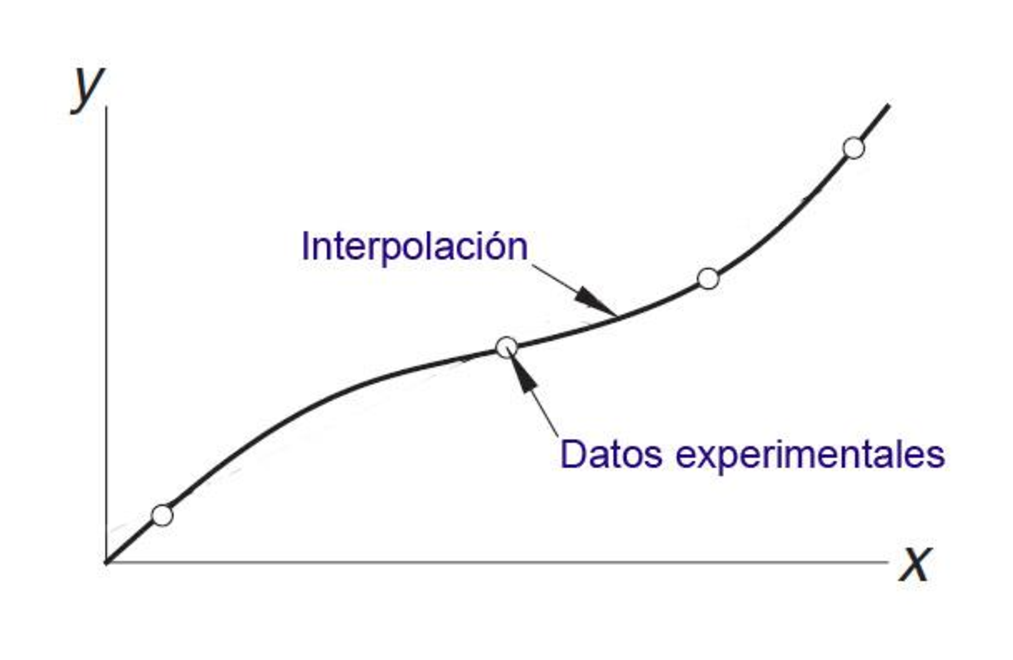
\includegraphics[scale=0.5]{Imagenes/Interpol02.eps}
\end{figure}
\end{frame}
\begin{frame}
\frametitle{Diferencia entre ajuste curvas e interpolación}
Ajuste de la curva:
\begin{figure}
   \centering
   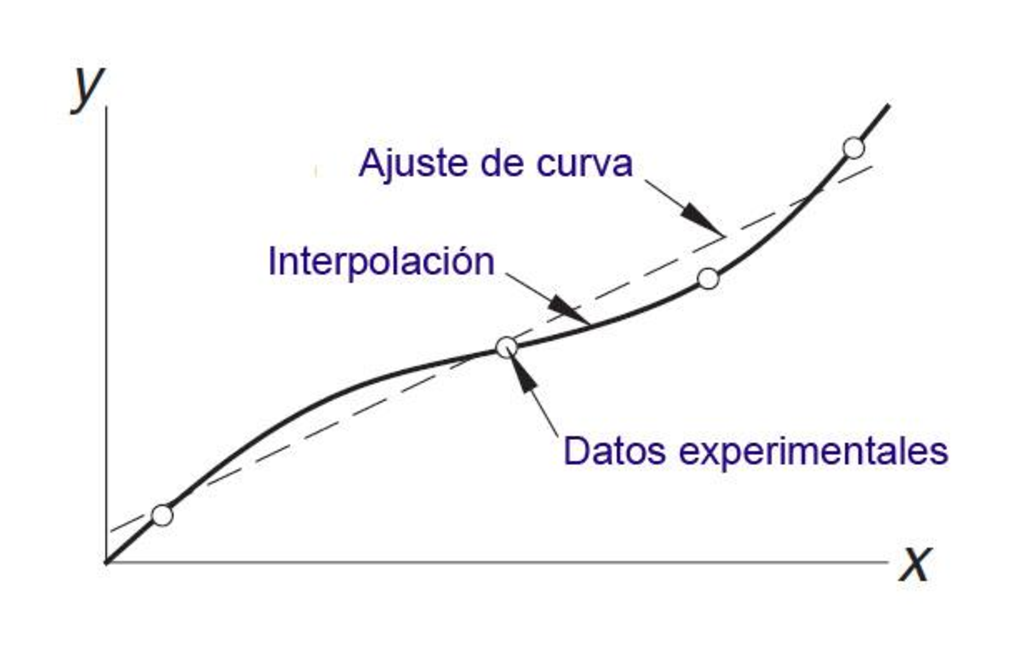
\includegraphics[scale=0.5]{Imagenes/Interpol03.eps}
\end{figure}
\end{frame}
\begin{frame}
\frametitle{Polinomio de interpolación}
Supongamos que lo que se quiere es buscar un polinomio de grado finito que aproxime una función dada.
\\
\bigskip
\pause
Lo que resulta intuitivo es buscar que dicho polinomio tenga el mismo valor de la función en un conjunto de puntos dado.
\end{frame}
\begin{frame}
\frametitle{Polinomio de interpolación}
Sabiendo que por $n$ puntos pasa un único polinomio de grado $n-1$, podríamos argumentar que la única manera de buscar una aproximación mejor del polinomio a la función es la de escoger de formas distintas los puntos por los cuales el polinomio ha de pasar.
\end{frame}
\begin{frame}
\frametitle{Polinomio de interpolación}
Dada una función $f(x)$ de la cual se conocen sus valores en un número finito de puntos $x_{0}, x_{1}, \ldots, x_{m}$, se llama \emph{interpolación polinómica} al proceso de hallar un polinomio $p_{m}(x)$ de grado menor o igual a $m$, cumpliendo $p_{m}(x_{k}) = f(x_{k})$ parar cada $k = 1, 2, \ldots, m$.
\end{frame}
\begin{frame}
\frametitle{Polinomio de interpolación}
Los coeficientes $a_{0}, a_{1}, a_{2}, \ldots, a_{n}$, de dicho polinomio se obtienen imponiendo al polinomio de pasar por los puntos fijados.
\end{frame}
\begin{frame}
\frametitle{Sistema matricial}
\begin{align*}
\mqty[
x_{0}^{n} & x_{0}^{n-1} & x_{0}^{n-2} & \ldots & x_{0} & 1 \\
x_{1}^{n} & x_{1}^{n-1} & x_{1}^{n-2} & \ldots & x_{1} & 1 \\
\vdots & \vdots & \vdots & & \vdots & \vdots \\
x_{n}^{n} & x_{n}^{n-1} & x_{n}^{n-2} & \ldots & x_{n} & 1 
]
\mqty[
a_{n} \\ a_{n-1} \\ \vdots \\ a_{0}
]
=
\mqty[
y_{0} \\ y_{1} \\ \vdots \\ y_{n}
]
\end{align*}
\pause
Este sistema es compatible y a la matriz asociada se le suele denominar \emph{matriz de Vandermonde}.
\end{frame}
\begin{frame}
\frametitle{Complejidad computacional}
La complejidad computacional para invertir la matriz es de $\order{n^{3}}$.
\\
\bigskip
\pause
Por esta razón, han sido construidos diferentes algoritmos que aprovechan la particular estructura de este sistema que reducen la complejidad a $\order{n^{2}}$, como el \emph{método de Lagrange} o el \emph{método de las diferencias divididas de Newton}.
\end{frame}
\section{Interpolación de Lagrange}
\frame{\tableofcontents[currentsection, hideothersubsections]}
\subsection{El método}
\begin{frame}
\frametitle{El método de Lagrange}
El polinomio interpolador de grado $n$ de Lagrange es un polinomio de la forma:
\begin{align*}
p_{n}(x) = \sum_{j=0}^{k} f_{j}(x) \, l_{j}(x) \hspace{1.5cm} n \leq m
\end{align*}
\end{frame}
\begin{frame}
\frametitle{Polinomios de Lagrange}
Donde los $l_{j}(x)$ son los llamados \emph{polinomios de Lagrange}, que se calculan como:
\fontsize{12}{12}\selectfont
\begin{eqnarray*}
&{}&l_{j}(x) = \prod_{j \neq i} \dfrac{x - x_{i}}{x_{j} - x_{i}} \\[0.5em]
&=& \dfrac{(x - x_{0})(x - x_{i}) \ldots(x - x_{j-1})(x - x_{j+1}) \ldots (x - x_{n})}{(x_{j} - x_{0})(x_{j} - x_{1}) \ldots(x_{j} - x_{j-1})(x_{j} - x_{j+1}) \ldots (x_{j} - x_{n})}
\end{eqnarray*}
\end{frame}
\begin{frame}
\frametitle{Ejemplo}
Se quiere hallar el valor de la función:
\begin{align*}
f(x) = e^{x+1}
\end{align*}
Utilizando un polinomio de interpolación de Lagrange de grado $2$ que pase por los puntos:
\pause
\fontsize{12}{12}\selectfont
\begin{table}
\centering
\begin{tabular}{c | c}
$x$ & $f(x)$ \\ \hline
$0$ & $f(0)$ \\
$0.5$ & $f(0.5)$ \\
$1$ & $f(1)$ \\
\end{tabular}
\end{table}
\end{frame}
\begin{frame}
\frametitle{Gráfica de los puntos}
Al graficar los puntos tendremos lo siguiente:
\begin{figure}
   \centering  
   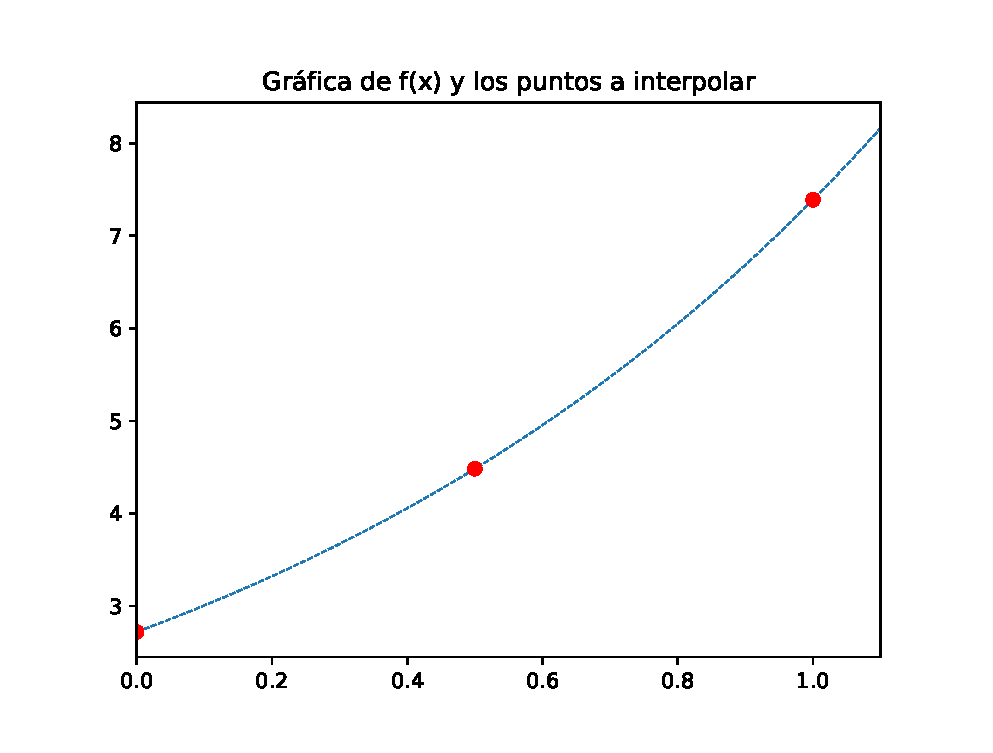
\includegraphics[scale=0.52]{Imagenes/Ejemplo_interpolacion_Chebychev_01.eps}
\end{figure}
\end{frame}
\begin{frame}
\frametitle{Obteniendo los polinomios}
Usamos el método directo para calcular el polinomio de interpolación. Con las condiciones dadas, los polinomios de Lagrange son:
\begin{align*}
l_{0} (x) &= \dfrac{(x - 0.5)(x - 1)}{0.5} = 2 \, x^{2} - 3 \, x + 1 \\[0.5em]
l_{1} (x) &= \dfrac{x (x - 1)}{-0.25} = - 4 \, x^{2} + 4 \, x \\[0.5em]
l_{2} (x) &= \dfrac{x (x - 0.5)}{0.5} = 2 \, x^{2} - x
\end{align*}
\end{frame}
\begin{frame}
\frametitle{Polinomio de interpolación}
El polimonio de interpolación de Lagrange de grado $2$ es:
\begin{align*}
p_{2}(x) &= \sum_{j=0}^{2} f_{j}(x) \, l_{j}(x) = \\[0.5em]
&= (2 \, e - 4 \, e^{3/2} + 2 \, e^{2}) \, x^{2} + \\[0.5em]
&+ (-3 \, - 4 \, e^{3/2} + 2 \, e^{2}) \, x + e
\end{align*}
\end{frame}
\begin{frame}
\frametitle{Error de la aproximación}
Una pregunta que puede surgir al utilizar un polinomio de interpolación para aproximar una función es qué tan bueno es el ajuste del polinomio a la función originaria.
\end{frame}
\begin{frame}
\frametitle{Error de la aproximación}
Por esta razón consideramos el error de interpolación de un polinomio de grado $n$ que pase por los puntos de una función $f(x)$ en los puntos $x_{0}, \ldots, x_{n}$.
\end{frame}
\begin{frame}
\frametitle{Error de la aproximación}
Si $f(x)$ es una función determinada en $x_{0}, \ldots, x_{n}$ y es $n$ veces diferenciable, entonces el \emph{error de interpolación} puede calcularse como valor absoluto de la diferencia entre la función y el polinomio.
\end{frame}
\begin{frame}
\frametitle{Error de la aproximación}
Construimos una función $\phi(x)$ por la cual se cumpla que
\begin{align*}
&\phi(x) = f(x) {-} p_{n}(x) {-} a(x)(x {-} a_{0})(x {-} a_{1}) \ldots (x {-} a_{n}) \\[0.5em]
&\exists \, \bar{x} \in [-1, 1] \\[0.5em]
&a(\bar{x}) = \big[ f(x) {-} p_{n} \big] (x {-} a_{0})(x {-} a_{1}) \ldots (x {-} a_{n}) = 0
\end{align*}
\end{frame}
\begin{frame}
\frametitle{Error de interpolación}
Esta función se anula en $n + 2$ puntos. Aplicando el \emph{teorema de Rolle} se tiene que una función que toma el mismo valor $n + 2$ veces tiene $n + 1$ puntos que anulan la derivada.
\end{frame}
\begin{frame}
\frametitle{Error de interpolación}
A la vez, la derivada de esta función es tal que, teniendo $n + 1$ puntos con el mismo valor tendrá $n$ puntos que anulan su derivada. 
\end{frame}
\begin{frame}
\frametitle{Error de interpolación}
Por lo tanto, derivando sucesivamente $n + 1$ veces, tenemos que existirá un único punto $\zeta$ que anule la derivada $n+1$-ésima, es decir:
\begin{align*}
\phi^{n+1} \, (\zeta) = 0
\end{align*}
\end{frame}
\begin{frame}
\frametitle{Error de interpolación}
Así podemos asegurar que $\phi^{n+1}$ tiene al menos una raíz, con lo cual resulta evidente que, siendo $p_{n}(x)$ un polinomio de grado mayor que $n‐1$, $\phi^{n+1} \, (\zeta)$ resultará la siguiente.
\begin{align*}
\phi^{n+1} \, (x) = f^{(n+1)} \, (\bar{x}) - a (\bar{x}) (n + 1)!
\end{align*}
\end{frame}
\begin{frame}
\frametitle{Error de interpolación}
Por consiguiente, al haber dejado que en $\phi^{n+1} \, (\bar{x}) = 0$, se tiene que:
\begin{align*}
a (\bar{x}) = \dfrac{f^{(n+1)} \, (\bar{x})}{(n + 1)!}
\end{align*}
\end{frame}
\begin{frame}
\frametitle{Error de interpolación}
En el caso de que $f(x)$ sea $n$ veces diferenciable en el dominio $[-1, 1]$, el error de interpolación podrá definirse como:
\begin{align*}
f(x) - p_{n}(x) = \dfrac{f^{(n+1)}(\xi)}{(n + 1)!} \, \prod_{i} (x - x_{i})
\end{align*}
\pause
Donde $\xi$ es un punto que pertenece a $[-1, 1]$, por lo cual $\phi^{(n+1)}(\zeta) = 0$.
\end{frame}
\begin{frame}
\frametitle{Maximizando la expresión}
Adjudicando valores absolutos en la expresión del error de interpolación y maximizando ambos lados de la desigualdad a lo largo del intervalo $[-1, 1]$ obtenemos la cota para dicho error:
\begin{align*}
&\max_{\abs{x} < 1} \abs{f(x) - p_{n}(x)} = \abs{\dfrac{f^{(n+1)}(\xi)}{(n + 1)!} \, \prod_{i} (x - x_{i})} \leq \\[0.5em]
&\leq \dfrac{\displaystyle \max_{\abs{x} < 1} \abs{f^{(n+1)}(\xi)}}{(n+1)!} \, \max_{\abs{x} < 1} \prod_{i} (x - x_{i})
\end{align*}
\end{frame}
\begin{frame}
\frametitle{Resultado del error}
Dada la unicidad del polinomio de interpolación, las únicas dos cosas que podemos mover a la hora de reducir el error de interpolación es el grado del polinomio (por consiguiente, el número de puntos) y la localización de dichos puntos.
\end{frame}
\begin{frame}
\frametitle{Resultado del error}
Se podría creer que al aumentar el grado del polinomio el error de interpolación se reduzca. 
\\
\bigskip
\pause
En realidad, pese al ser un resultado antiintuitivo, Carle David Tolmé Runge observó que el error de interpolación en un intervalo dado, tiende a infinito cuando el grado del polinomio de interpolación tiende a infinito.
\end{frame}
\begin{frame}
\frametitle{Resultado del error}
Es decir:
\begin{align*}
\lim_{n \to \infty} \big( \max_{\abs{x} < 1} \abs{f(x) - p_{n}(x)} \big) = \infty
\end{align*}
\end{frame}
\begin{frame}
\frametitle{Error mínimo}
El método que veremos nos permite proporcionar los puntos por los cuales hacer pasar el polinomio de interpolación de forma tal que la distancia máxima entre el polinomio interpolado y la función originaria sea mínima.
\end{frame}
\begin{frame}
\frametitle{Error mínimo}
La oscilación observada por Runge se puede minimizar usando nodos de Chebyshev en lugar de nodos equidistantes.
\\
\bigskip
\pause
En este caso se garantiza que el error máximo disminuye al crecer el orden polinómico.
\end{frame}
\section{Polinomios de Chebychev}
\frame{\tableofcontents[currentsection, hideothersubsections]}
\subsection{Usando las raíces}
\begin{frame}
\frametitle{Raíces de los polinomios}
Esta es una propiedad que hace particularmente interesante el utilizar las raíces de los polinomios de Chebyshev como puntos por donde interpolar el polinomio.
\end{frame}
\begin{frame}
\frametitle{Minimizando el error}
Para minimizar el último factor de la cota del error, Pafnuty Lvovich Chebyshev demostró que los puntos $x_{0}, \ldots, x_{n}$ por los cuales hacer pasar el polinomio, han de ser escogidos de forma que:
\begin{align*}
\max_{\abs{x}<1} \prod_{i} (x - x_{i}) = \dfrac{1}{2^{n}} \, T_{n+1} (x)
\end{align*}
donde $T_{n+1}(x)$ es el polinomio de Chebychev de primera clase de orden $n + 1$.
\end{frame}
\begin{frame}
\frametitle{Elección de los puntos}
Entre todas las elecciones de los puntos $x_{0}, \ldots, x_{n}$, elegirlos de forma que la siguiente expresión se respete:
\begin{align*}
\phi^{n+1} \, (x) = f^{(n+1)} \, (\bar{x}) - a (\bar{x}) (n + 1)!
\end{align*}
\end{frame}
\begin{frame}
\frametitle{Elección de los puntos}
Se garantiza que el polinomio así obtenido es el polinomio único que tenga la propiedad:
\begin{align*}
\max_{\abs{x}<1} T_{n} (x) &\leq \max_{\abs{x}<1} \prod (x - x_{i}) \\[0.5em]
\max_{\abs{x}<1} T_{n} (x) &= \dfrac{1}{2^{n}} \\[0.5em]
\dfrac{1}{2^{n}} &\leq \max_{\abs{x}<1} T_{n} (x)
\end{align*}
\end{frame}
\begin{frame}
\frametitle{Error de interpolación}
Se puede demostrar que el valor absoluto de la diferencia entre la función y el polinomio interpolado por las raíces del polinomio de Chebyshev resulta acotado de la siguiente forma:
\begin{align*}
\abs{f(x) - p_{n-1}} \leq \dfrac{1}{2^{n-1} \, n!} \, \max_{\xi \in [-1, 1]}  \, \abs{f^{n} \, (\xi)}
\end{align*}
\end{frame}
\end{document}